%!TEX root = ../../main.tex

\begin{figure}[p]
    \centering
    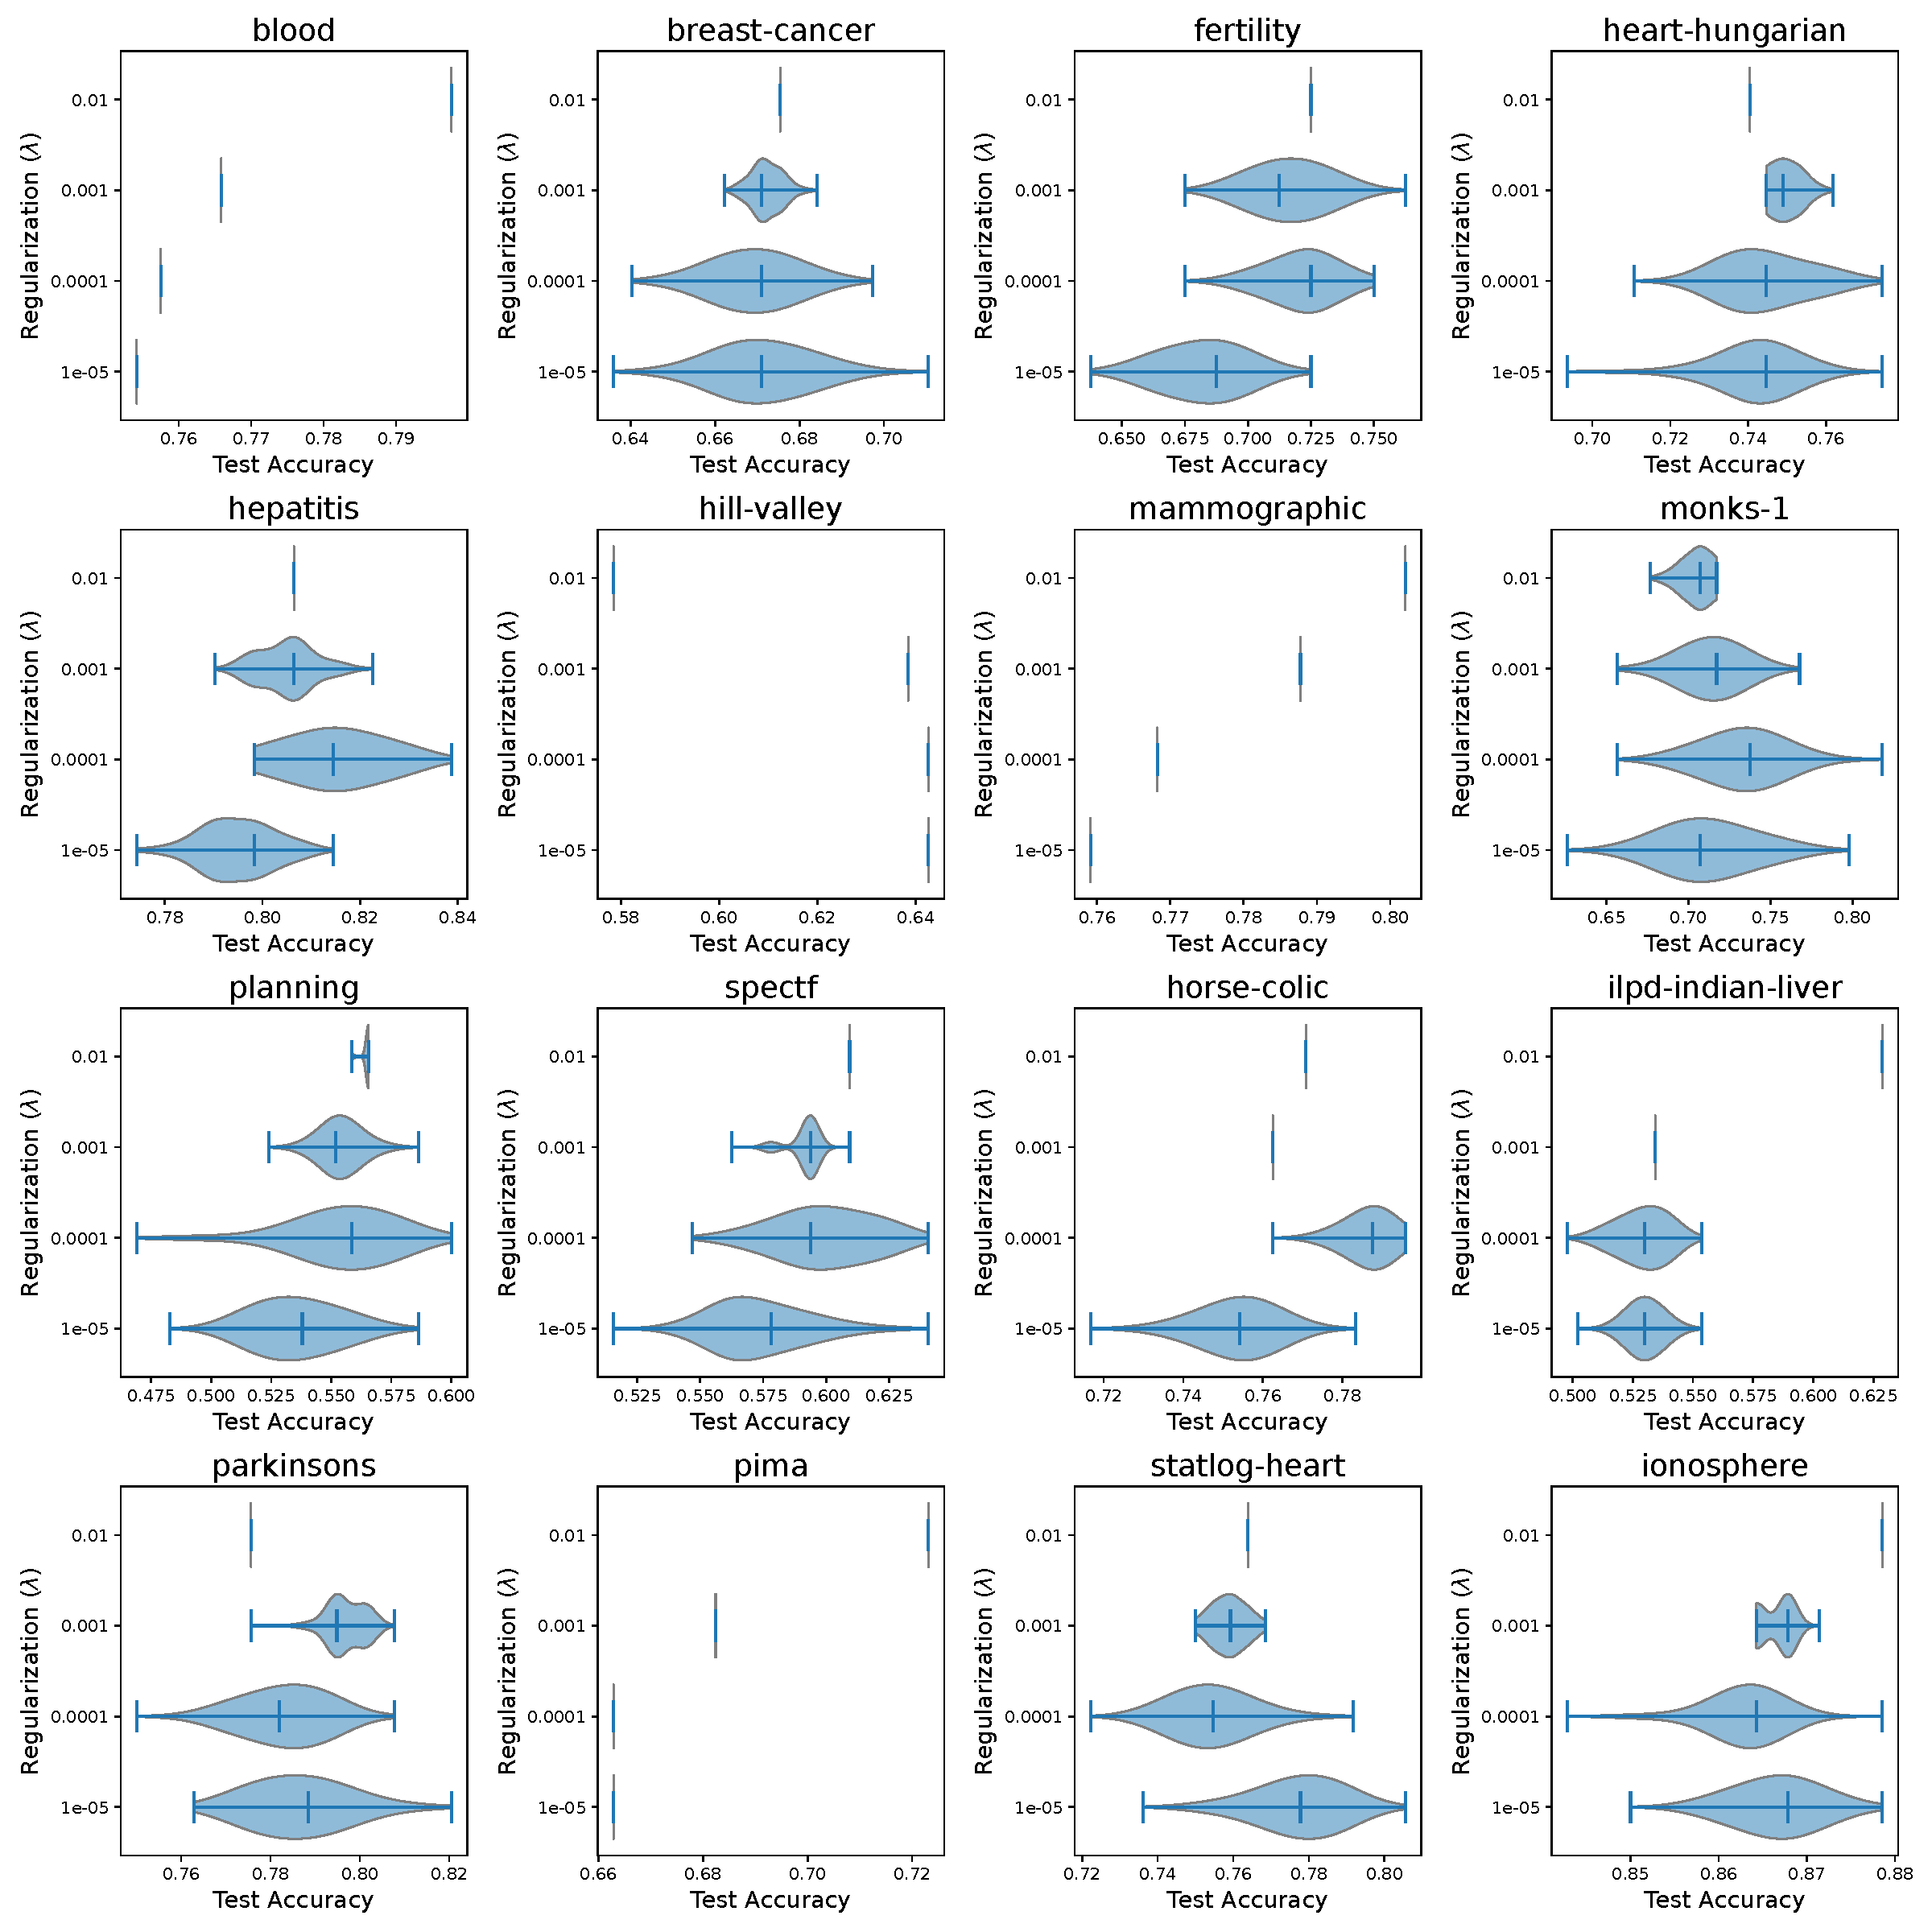
\includegraphics[width=0.98\textwidth]{figures/chapter_three/test_dist_appendix.pdf}
    \caption{Distribution of test accuracy over 10,000 uniform samples taken
        from the optimal sets for two-layer ReLU networks on \( 16 \) datasets
        from the UCI repository.
        The majority of datasets (\( 11 / 16 \)) show non-negligible variation
        in generalization performance over the optimal set, particular for
        small regularization parameters.
        This is particularly true for the \texttt{breast-cancer},
        \texttt{spectf}, and \texttt{fertility} datasets, addition to the
        \texttt{monks-1} and \texttt{planning} datasets shown in the main paper.
        The remaining five datasets show little-to-no different in test
        performance over the optimal set;
        note that this does not imply the optimal set is a singleton (i.e.
        that the global minimum is unique), but only that global minima
        have the test test performance.
    }%
    \label{fig:uci-sampling-full}
\end{figure}

\begin{figure}[t]
    \centering
    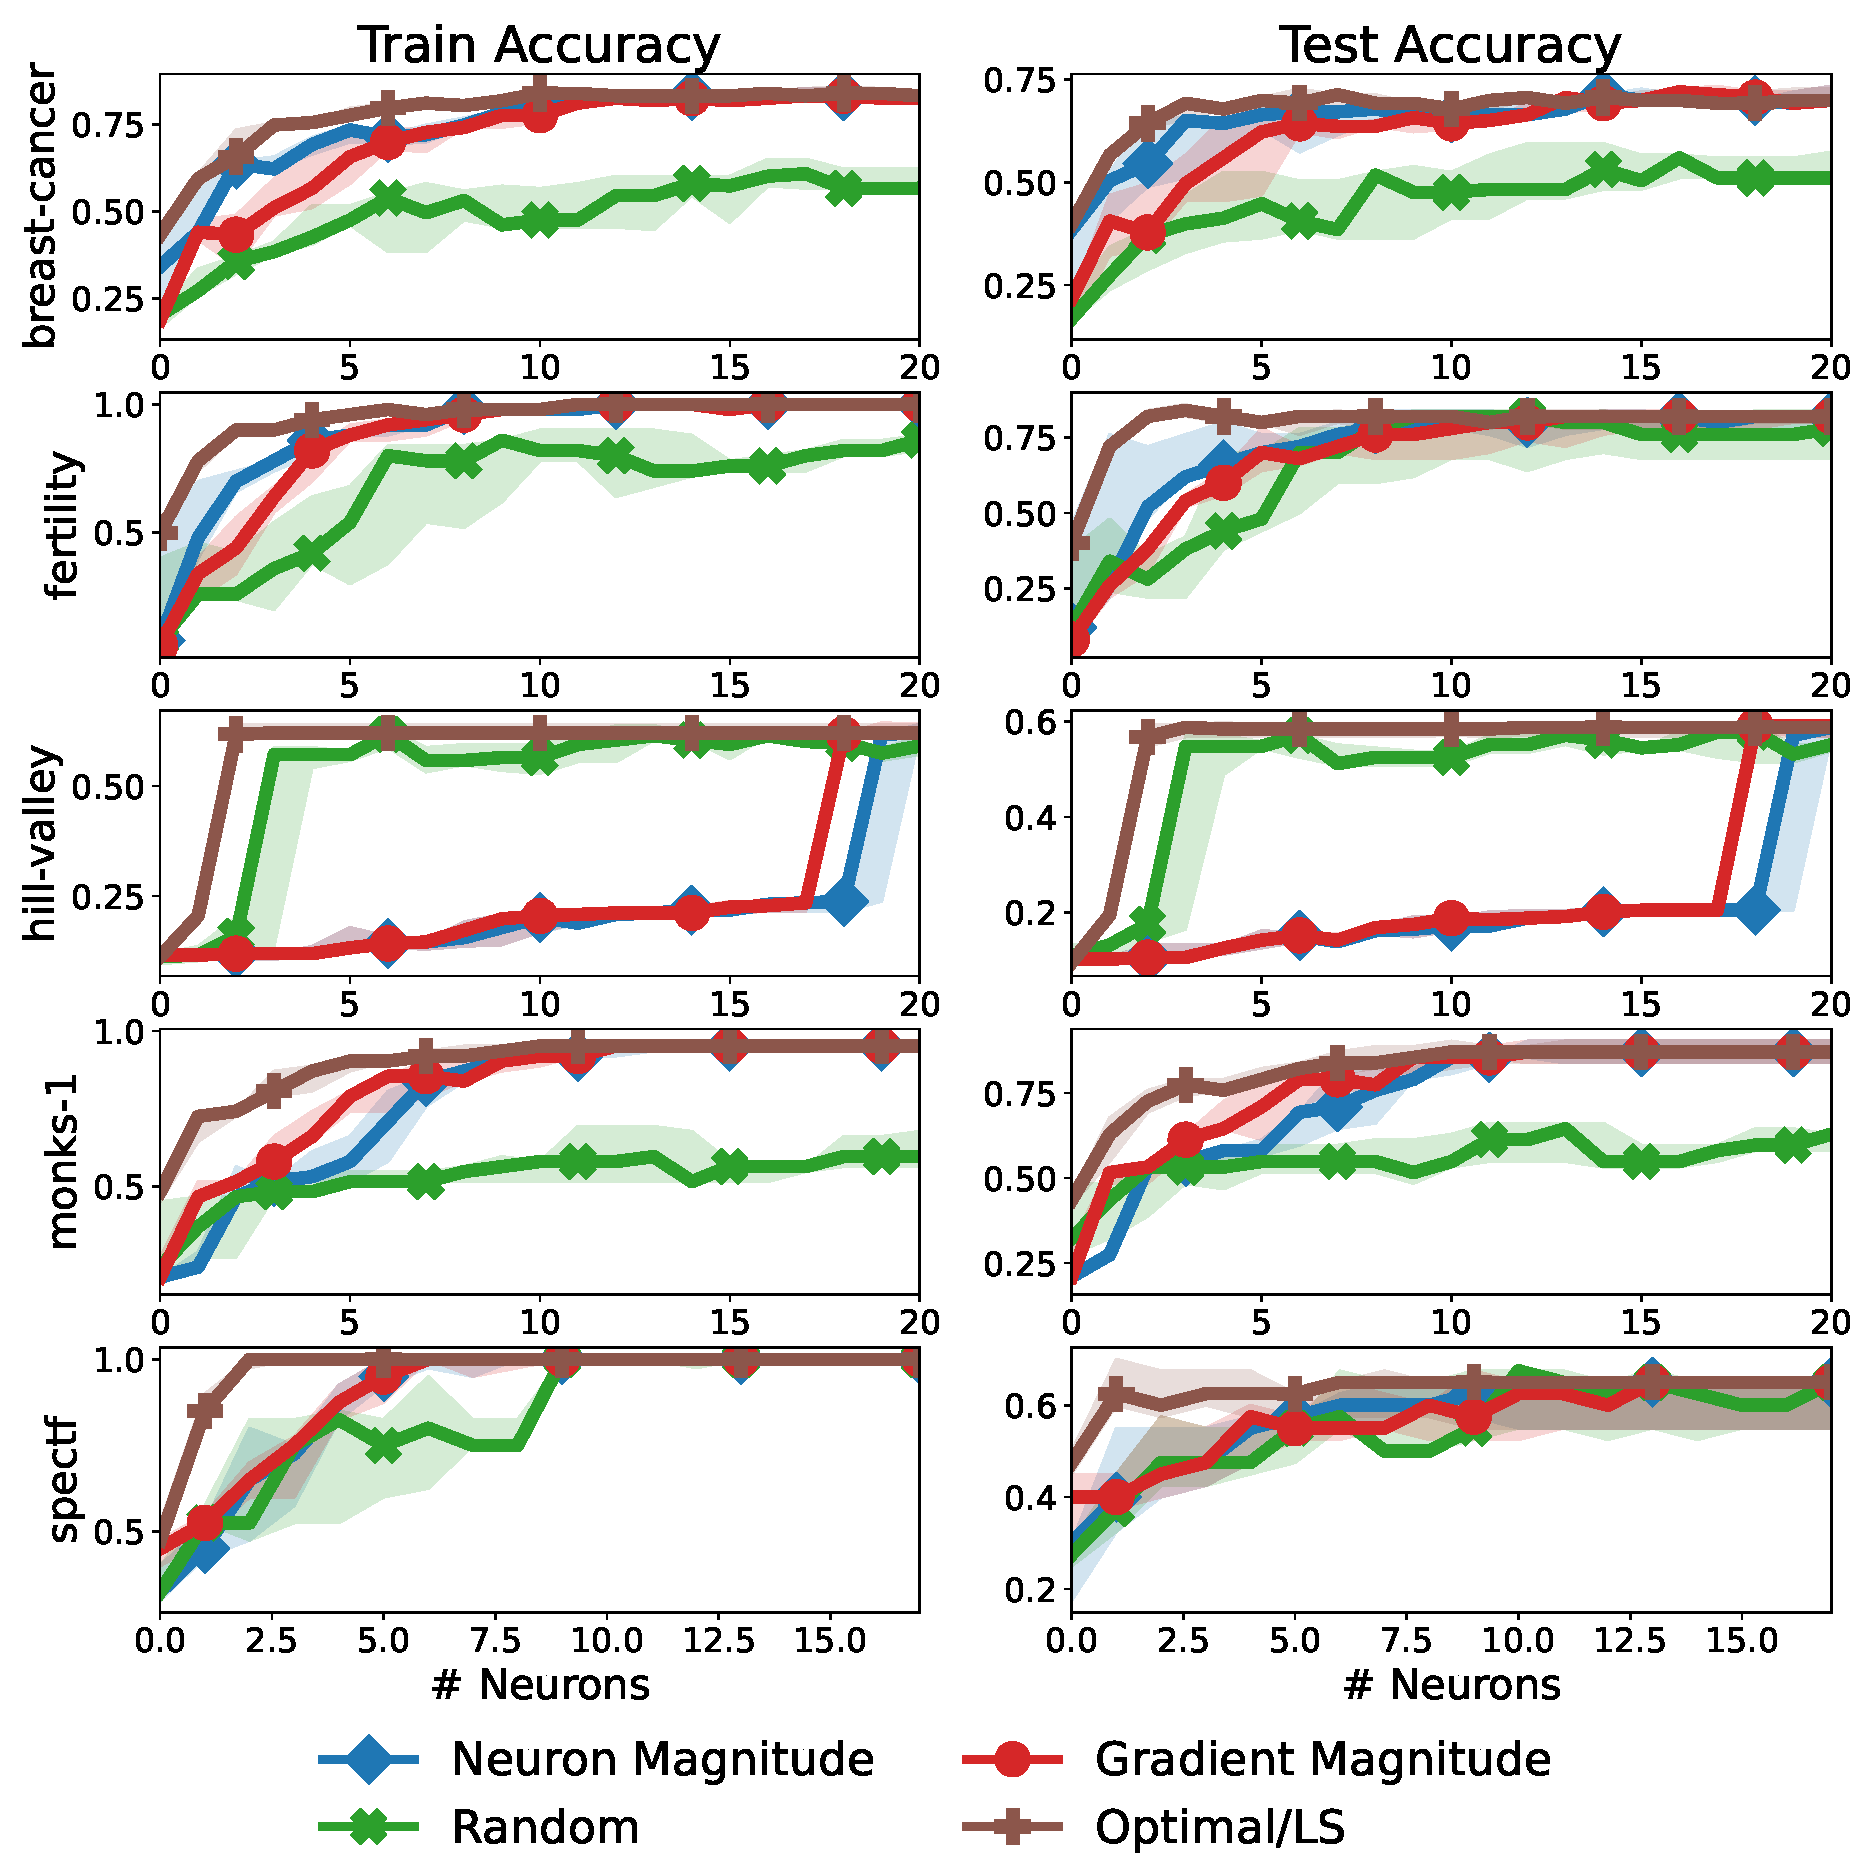
\includegraphics[width=0.7\textwidth]{figures/chapter_three/uci_pruning_full_paper.pdf}
    \caption{Pruning neurons on five datasets from the UCI repository.
        This figure extends \cref{fig:uci-pruning-acc} with training
        accuracy in addition to the test accuracies shown in the main paper.
    }%
    \label{fig:uci-pruning-full}
\end{figure}

\begin{figure}[t]
    \centering
    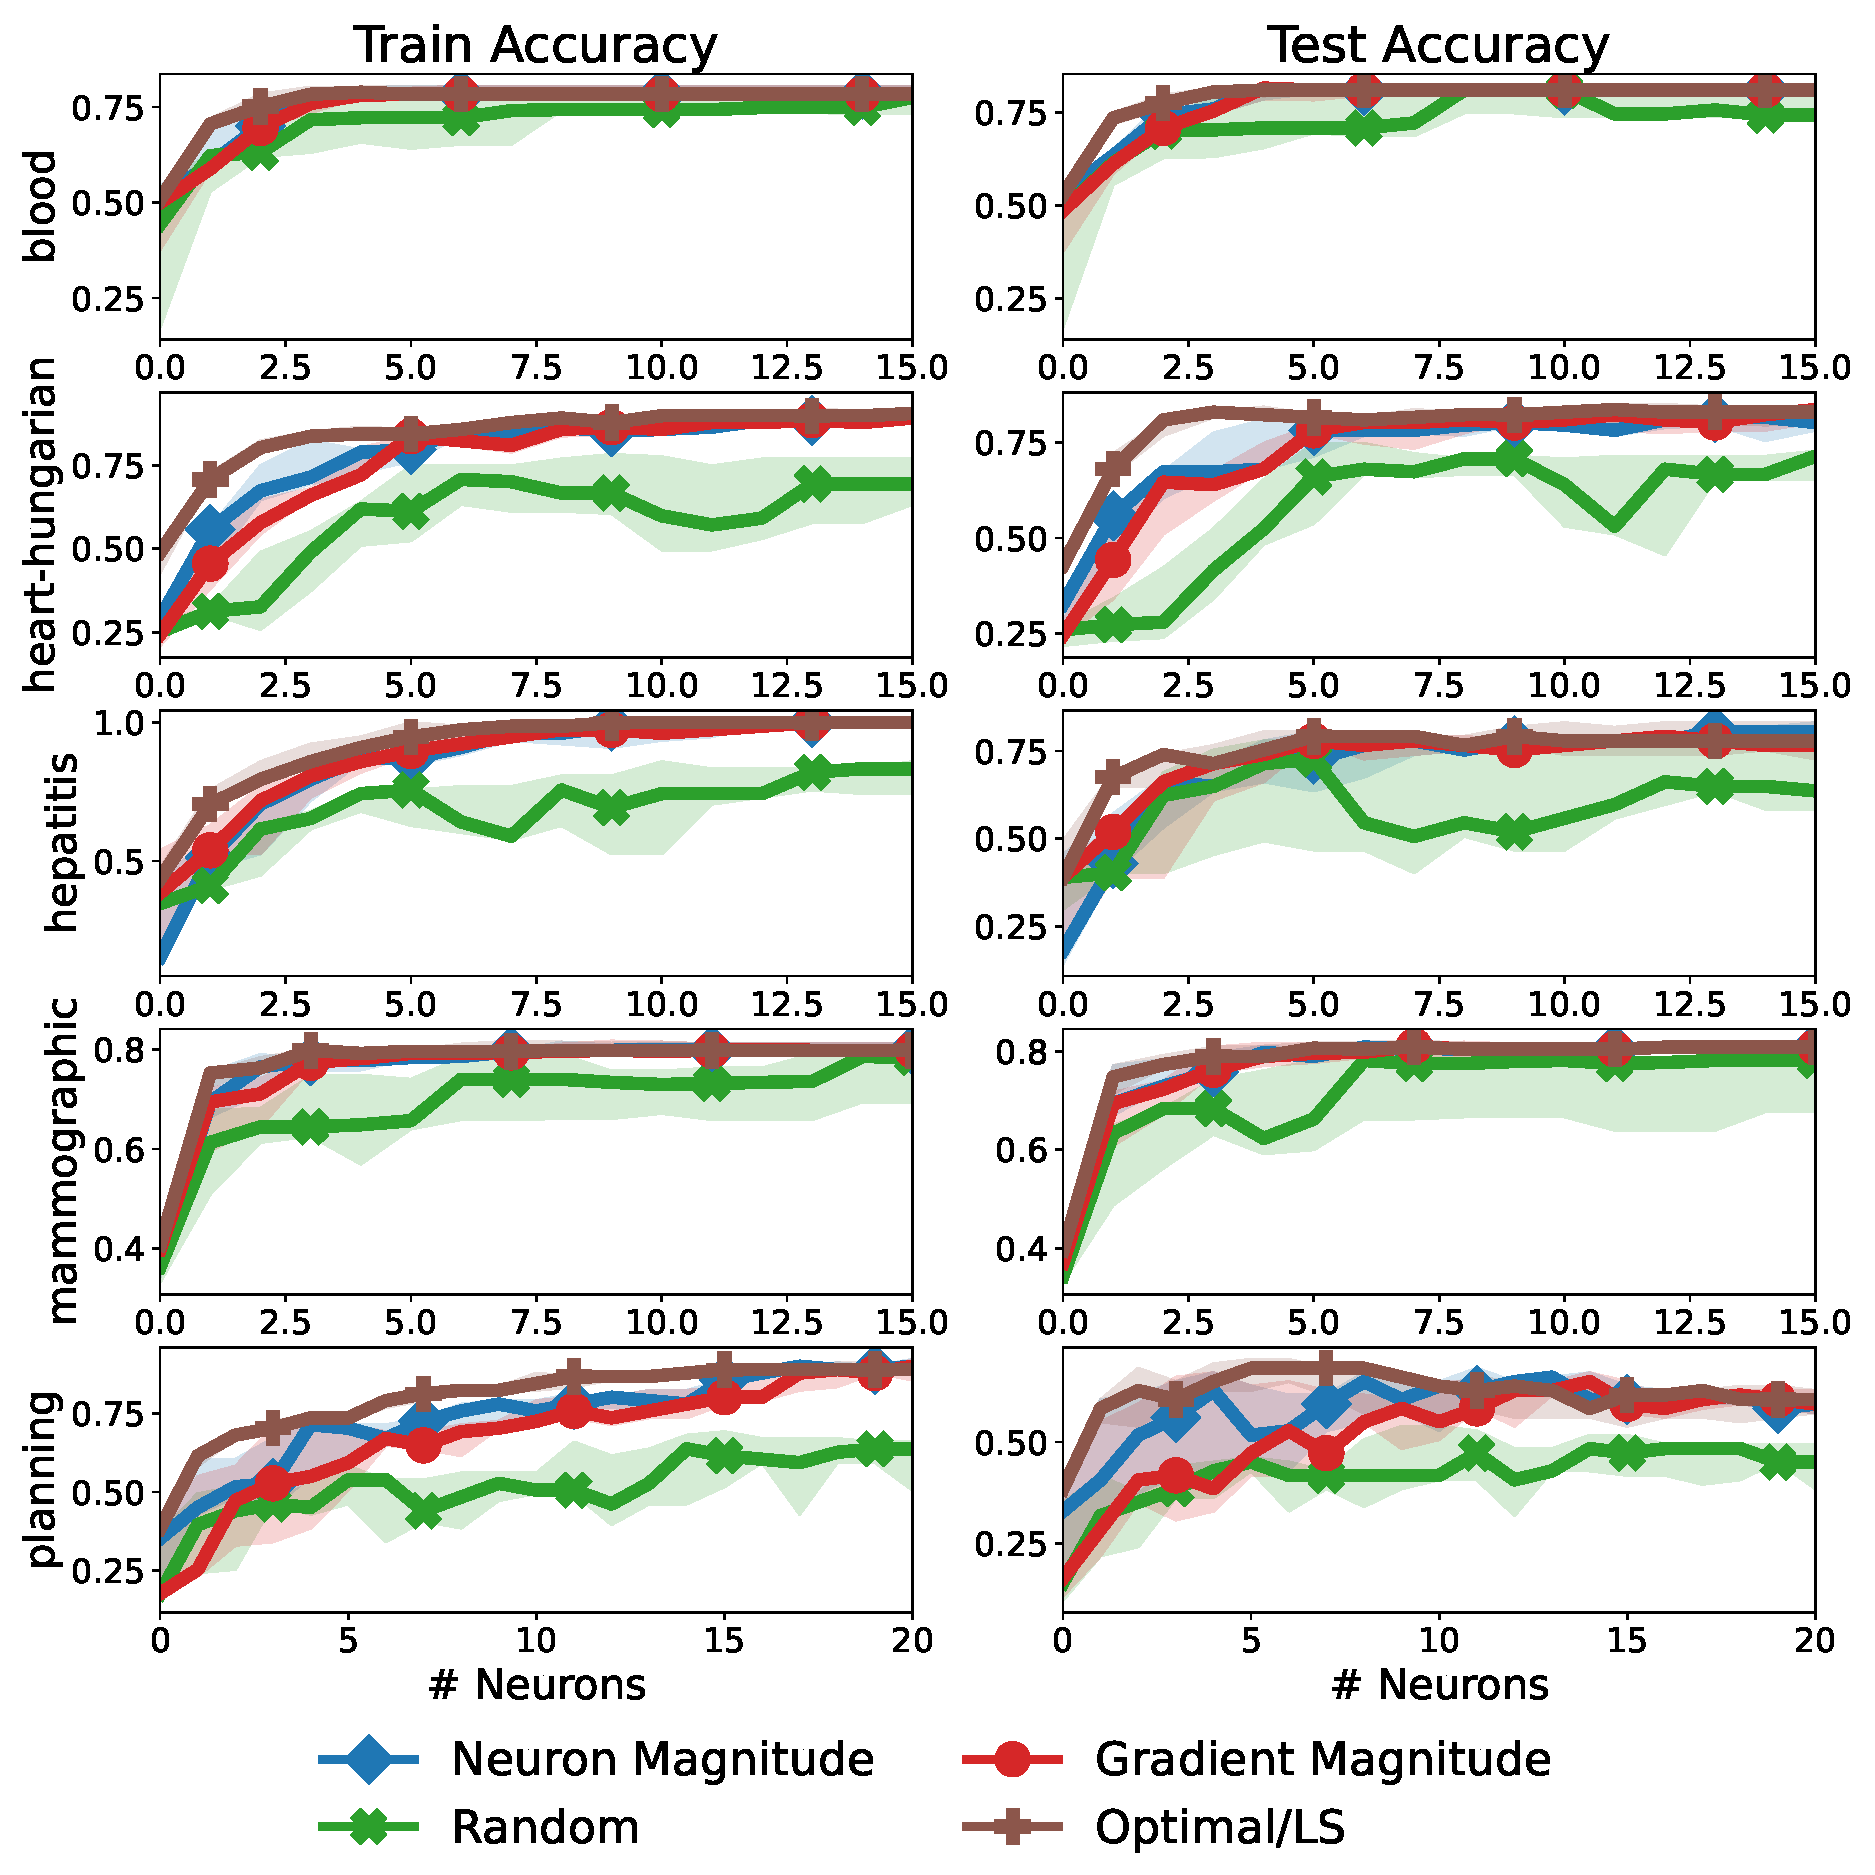
\includegraphics[width=0.8\textwidth]{figures/chapter_three/uci_pruning_full_appendix.pdf}
    \caption{Pruning neurons on five additional datasets from the UCI repository.
        See \cref{fig:uci-pruning-acc} for details.
        Our method (\textbf{Optimal/LS}) preservers test accuracy for longer
        than the baseline methods, leading to compact models with better
        generalization.
    }%
    \label{fig:uci-pruning-appendix}
\end{figure}

In this section we provide additional experimental results as well as
the necessary details to replicate our pruning experiments.
Code to replicate all of our experiments is provided at
\url{https://github.com/pilancilab/relu_optimal_sets}.

\subsection{Additional Results}

\begin{figure}[p]
    \centering
    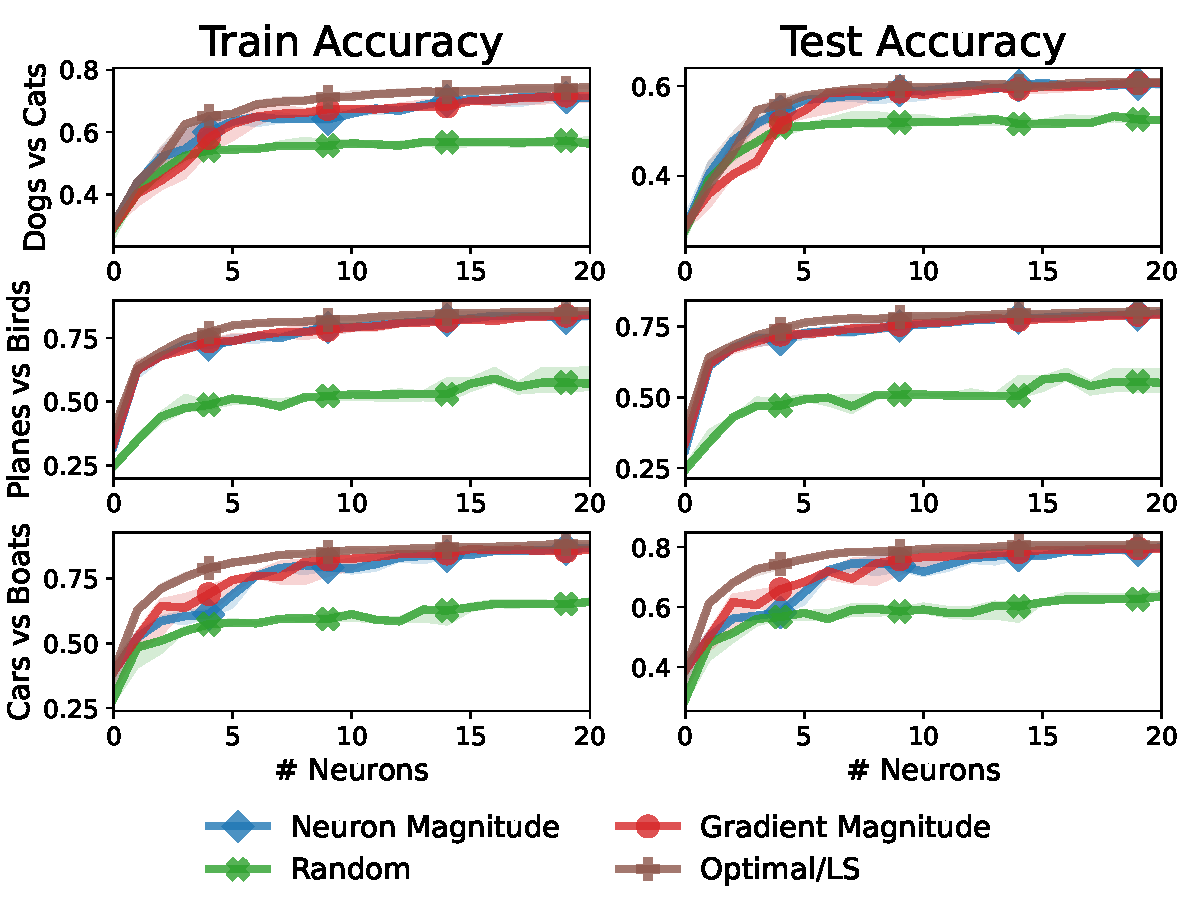
\includegraphics[width=0.8\textwidth]{figures/chapter_three/cifar_pruning_full.pdf}
    \caption{Pruning experiments on binary classification tasks
        from the CIFAR-10 dataset.
        This figure reproduces results from \cref{fig:cifar-pruning-acc}
        with training accuracies added and also includes results for
        an additional task,
        \texttt{cats vs dogs}, not presented in the main paper.
    }%
    \label{fig:cifar-pruning-full}
\end{figure}

\begin{figure}[p]
    \centering
    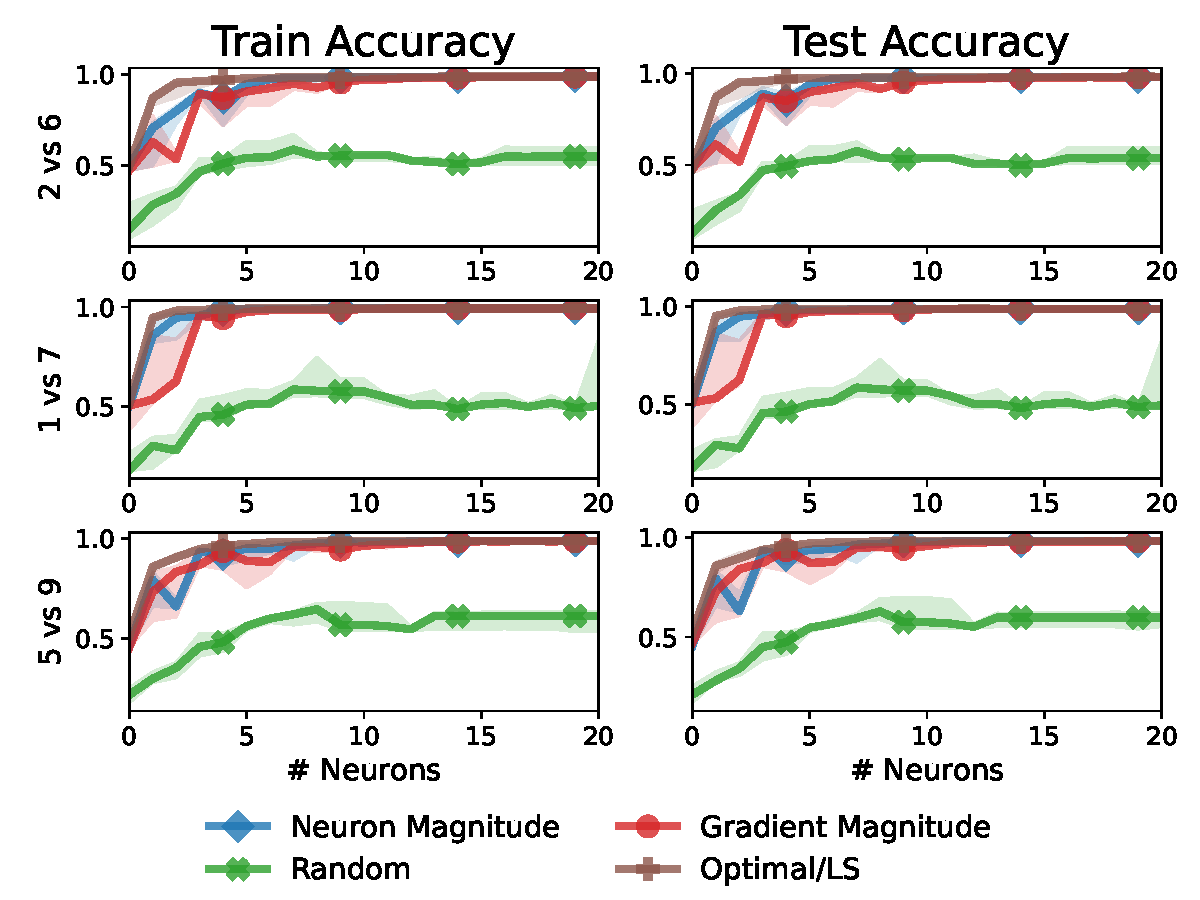
\includegraphics[width=0.8\textwidth]{figures/chapter_three/mnist_pruning_full.pdf}
    \caption{Pruning experiments on three binary classification tasks
        taken from MNIST.
    }%
    \label{fig:mnist-pruning-full}
\end{figure}

\setlength{\tabcolsep}{2pt} % Default value: 6pt

\begin{table}[t]
    \centering
    \caption{Tuning neural networks by searching over the optimal set.
        We fit two-layer ReLU networks on the training set and
        compute the minimum \( \ell_2 \) norm solution (Min L$_2$).
        Then we tune by finding an extreme point approximating
        the maximum \( \ell_2 \)-norm solution (EP), minimizing validation
        MSE over the optimal set (V-MSE), and minimizing test MSE over
        the optimal set (T-MSE).
        Max Diff. reports the difference between the best and worse models
        found.
        For each method we give the median and interquartile range as
        \texttt{median (lower/upper)}.
    }
    \small
    \label{table:tuning-full}
    \vspace{0.1in}
    \begin{tabular}{lccccc} \toprule
        \textbf{Dataset}  & \textbf{Min L$_2$} & \textbf{EP}      & \textbf{V-MSE}   & \textbf{T-MSE}   & \textbf{Max Diff.} \\
        \midrule
        blood             & 0.72 (.72/.74)   & 0.72 (.72/.74) & 0.62 (.61/.62) & 0.7 (.68/.71)  & 0.1 (.11/.12)    \\
        breast-c.     & 0.64 (.61/.65)   & 0.64 (.61/.65) & 0.61 (.6/.64)  & 0.71 (.66/.71) & 0.1 (.06/.08)    \\
        fertility         & 0.66 (.62/.7)    & 0.69 (.62/.69) & 0.65 (.64/.7)  & 0.64 (.57/.64) & 0.05 (.06/.06)   \\
        heart-h.   & 0.75 (.7/.77)    & 0.75 (.7/.77)  & 0.71 (.56/.72) & 0.85 (.82/.86) & 0.14 (.26/.14)   \\
        hepatit.         & 0.75 (.74/.78)   & 0.75 (.74/.78) & 0.73 (.69/.75) & 0.77 (.77/.9)  & 0.05 (.08/.15)   \\
        hill-va.       & 0.64 (.64/.65)   & 0.65 (.64/.65) & 0.64 (.64/.67) & 0.64 (.64/.65) & 0.0 (.0/.01)     \\
        mammo.      & 0.77 (.77/.77)   & 0.77 (.77/.77) & 0.57 (.56/.62) & 0.78 (.78/.8)  & 0.21 (.22/.18)   \\
        monks-1           & 0.67 (.64/.71)   & 0.66 (.64/.71) & 0.49 (.48/.51) & 0.57 (.51/.61) & 0.17 (.15/.2)    \\
        planning          & 0.53 (.51/.61)   & 0.52 (.51/.61) & 0.53 (.52/.53) & 0.7 (.68/.74)  & 0.17 (.17/.21)   \\
        spectf            & 0.64 (.62/.7)    & 0.64 (.62/.7)  & 0.56 (.53/.56) & 0.58 (.56/.66) & 0.08 (.09/.14)   \\
        horse-c.       & 0.75 (.75/.76)   & 0.59 (.57/.61) & 0.74 (.73/.75) & 0.85 (.85/.85) & 0.26 (.27/.24)   \\
        ilpd-in. & 0.59 (.57/.6)    & 0.59 (.57/.6)  & 0.53 (.53/.57) & 0.72 (.7/.73)  & 0.19 (.17/.17)   \\
        parkins.        & 0.74 (.72/.74)   & 0.74 (.72/.74) & 0.65 (.65/.74) & 0.88 (.86/.9)  & 0.23 (.21/.16)   \\
        pima              & 0.68 (.66/.68)   & 0.68 (.66/.68) & 0.68 (.64/.7)  & 0.87 (.86/.88) & 0.2 (.22/.19)    \\
        tic-ta.       & 0.98 (.98/.98)   & 0.76 (.69/.8)  & 0.98 (.98/.99) & 1.0 (1.0/1.0)    & 0.24 (.31/.2)    \\
        statlo.     & 0.71 (.7/.73)    & 0.71 (.7/.73)  & 0.7 (.67/.73)  & 0.84 (.83/.86) & 0.14 (.17/.13)   \\
        ionosp.        & 0.85 (.83/.86)   & 0.76 (.73/.76) & 0.84 (.84/.84) & 0.88 (.88/.89) & 0.12 (.15/.12)   \\
        \bottomrule
    \end{tabular}
\end{table}

\setlength{\tabcolsep}{6pt} % Default value: 6pt


\textbf{Tuning} \cref{table:tuning-full} shows results for our tuning
task on an additional 7 datasets, as well as the 10 given in \cref{table:tuning-small}.
We report the interquartile range as well as median test accuracies for each
method.
We observe similar results as presented in the main text.
Only one dataset (\texttt{tic-tac-toe}) shows no variation in test
accuracy as we explore the optimal set.

\textbf{Sampling}: \cref{fig:uci-sampling-full} shows the full results
of sampling from the set of optimal two-layer ReLU networks for \( 16 \)
datasets taken from UCI repository.
While the results for \texttt{monks-1} and \texttt{planning} shown in the
main paper are the most striking, \( 11 / 16 \) datasets show significant
variation in the test performance of different optimal neural networks.

\textbf{Pruning}: \cref{fig:uci-pruning-full} shows train and test
accuracy for our
optimal/least-squares pruning method as well as magnitude/gradient-based pruning
and random pruning on the same five datasets from the UCI repository as
presented in \cref{fig:uci-pruning-acc}.
Our approach shows significantly less decay in train accuracy as neurons are
pruned; this matches the intuition of the least-squares heuristic for pruning,
which selects the coefficients \( \beta \) to best preserve the model fit.

We observe that both our pruning method and pruning by neuron/gradient norm
show very similar training accuracy until most of the neurons have been pruned.
While this behavior is expected from our theory-based approach, it is somewhat
surprising that pruning by neuron/gradient-norm also maintains train accuracy
nearly as well.
This behavior suggests that there are many neurons with very small norm which
can be eliminated without significantly affecting the model prediction.

\cref{fig:uci-pruning-appendix} presents results for neuron pruning on
five additional datasets from the UCI repository, while
\cref{fig:mnist-pruning-full} shows results for three binary classification
tasks taken from the MNIST dataset.
The trends are generally the same as in \cref{fig:uci-pruning-full},
with our approach (\textbf{Theory/LS}) outperforming the baselines.
Finally \cref{fig:cifar-pruning-full} extends the results on CIFAR-10
given in \cref{fig:cifar-pruning-acc} with one additional task
and with training accuracies.

\subsection{Experimental Details}

Now we give the details necessary to reproduce our experiments.
Our experiments use the pre-processed versions of UCI datasets provided by
\citet{delgado2014hundreds}, but do we do not use their evaluation procedure as
it is known to have data leakage.

\subsubsection{Tuning}

We select 17 binary classification datasets from the UCI
repository.
For each dataset we use a random 60/20/20 split of the data
into train, validation, and test sets.
We use the commercial interior point method MOSEK \citep{aps2022mosek}
through the interface provided by CVXPY \citep{diamond2016cvxpy}
to compute the initial model which is then tuned.
We modify the tolerances of this method to use \( \tau = 10^{-8} \) for measuring
both primal convergence and violation of the constraints.
For each dataset, we use fixed \( \lambda = 0.001 \) and a maximum of 1000
neurons.
To compute the min \( \ell_2 \)-norm optimal model,
we use the MOSEK and the optimization problem given in \cref{prop:min-norm-program}.

To approximate the maximum \( \ell_2 \)-norm model, we solve the
following program:
\begin{equation*}
    \begin{aligned}
        \alpha^* = \argmax_{\alpha \geq 0} \sum_{\bi \in \calS_\lambda} \alpha_\bi
        \, \, \text{ s.t.} \, \,
        \sum_{\bi \in \calS_\lambda} \alpha_{\bi} \Xbi \vi = \hat y.
    \end{aligned}
\end{equation*}
This is a linear program which is straightforward to solve using
interior point methods.
Moreover, we have
\[
    \norm{w^*}_2^2 = \lambda^2 \sum_{\bi} (\alpha_\bi^*)^2,
\]
so that \( \sum_{\bi} \alpha_\bi \) acts as an approximation, where we recall
\( \alpha_\bi \geq 0 \) necessarily.

To tune each model with respect to the validation/test MSE, we solve the following optimization problem:
\[
    \min_{w} \cbr{ \half \norm{\tilde X w - \tilde y}_2^2 : w \in \solfn(\lambda) },
\]
with respect to the parameters of the convex formulation.
Here, \( (\tilde X, \tilde y) \) is either the validation or test
set.
We repeat each experiment five times with different random splits of the
data and random resamplings of \( 500 \) activation patterns \( D_i \).
This guarantees that each non-convex network has at most \( 1000 \) neurons
after optimization, although it may have less due to the sparsity inducing
penalty.

\subsubsection{Sampling}

We use the same 17 datasets from the UCI repository as in our tuning
experiments, but do not include results for \texttt{tic-tac-toe} because
they are uniformly the same for each regularization parameter.
We consider regularization parameters in the grid
\( \cbr{10^{-5}, 10^{-4}, 10^{-3}, 10^{-2}} \).
For each dataset-regularization parameter pair, we solve a sub-sampled convex
reformulation with \( 50 \) activation patterns using CVXPY
\citep{diamond2016cvxpy} and compute the optimal model fit and
block-correlation vectors using the resulting solution.
This allows us to describe the optimal set as a convex polytope from which
we sample using hit-and-run.
We use on the hit-and-run implementation available at
\url{https://github.com/fontclos/hitandrun}, but modify it to allow for
sampling from a polytope contained in a linear subspace
(i.e. a polytope with linear equality constraints).
Our code is available at \url{https://github.com/aaronpmishkin/hitandrun}.
Figures~\ref{fig:uci-sampling-paper} and~\ref{fig:uci-sampling-full}
are generated by taking \( 10,000 \) samples from the optimal set for each
problem and them plotting them with a smoothing parameter of \( 0.6 \).

For \cref{fig:uci-optimizer-sampling}, we consider running SGD and Adam
\( 1000 \) times with different random restarts to sample stationary
points of the training problem.
We restrict ourselves to the \texttt{monks-1} and \texttt{planning} datasets
and regularization strength of \( \lambda = 10^{-5} \)
since this operation is much more expensive than sampling from optimal set
using hit-and-run.
For both Adam and SGD, we use the step-size schedule
\( \eta_k = \eta_0 / k \) so that the methods can actually converge to a critical point.
The initial step-size \( \eta_0 \) was selected by grid-search over the set
\( \cbr{10^{-3}, 10^{-2}, 10^{-1}, 1} \).
For both datasets, we found that \( \eta_0 = 10^{-1} \) worked best
for SGD, while \( \eta_0 = 10^{-3} \) worked best for Adam.
For each dataset, we ran both methods for \( 10,000 \) epochs with batch size
of \( 25 \) samples.
We rejected a run of SGD or Adam if the final iterate had a pseudo-gradient
norm larger than \( 10^{-6} \).
For \texttt{monks-1}, this procedure resulted in 905 accepted samples for SGD
and only 358 accepted samples for Adam.
For \texttt{planning}, we obtained \( 1000 \) samples for SGD and \( 580 \)
for Adam.

\subsubsection{Pruning}

\textbf{Methods}:
We use the augmented Lagrangian method of \citet{mishkin2022convex} to compute
the starting model which is then pruned.
We modify the tolerances of this method to use \( \tau = 10^{-8} \) for measuring
both primal convergence and violation of the constraints.

Pruning by neuron magnitude is straightforward: we sort the neurons
by \( \norm{W^{(1)}_{\cdot, i} W^{(2)}_{i}}_2 \), which measures the total magnitude of the
neuron, and then drop the smallest one.
For pruning by gradient norm, we compute
\( G_{1i} = \nabla_{W^{(1)}_{\cdot, i}} \calL(f_{W^{(1)}, W^{(2)}}(Z), y) \),
\( g_{2i} = \nabla_{W_{2i}} \calL(f_{W^{(1)}, W^{(2)}}(Z), y) \) and then score each
neuron as
\[
    s_i = \norm{W^{(1)}_{\cdot, i} \cdot G_{1i} W^{(2)}_{i} g_{2i}}_2,
\]
where \( \cdot \) indicates the element-wise product.
The neuron with smallest score is zeroed.
This is consistent the existing implementations of pruning by
gradient norm \citep{bialock2020pruning} and attempts to measure the
variation of a linearization of the loss in neuron \( i \).
For Random, we simply select a neuron from a uniform random distribution.

For Optimal/LS, we start by using \cref{alg:pruning-solutions} to prune
until no linear dependence exists amongst the neuron fits \( D_i Z W^{(1)}_{\cdot, i} \).
At this point, we choose \( \beta \) to minimize the squared-error
in the training fit.
We choose the neuron to prune by selecting the index that minimizing the residual
in the least-squares fit,
\[
    i_k = \argmin_{j} \min_{\beta}
    \half \norm{\sum_{i \neq j} \beta_i D_i Z w_i  - D_j Z w_j}.
\]
This produced the best result in all of our experiments, although you can
also select \( i_k \) using neuron magnitude or any other rule in the literature
on structured pruning.

\textbf{UCI Datasets}:
We select 10 moderately-sized binary classification datasets from the UCI repository.
For each dataset we use a random 50/50 split of the data
into train and test sets,
fixed \( \lambda = 0.01 \), and sample 25
activation patterns \( D_i \).
This results in a maximum of 50 neurons in each final model;
since the datasets are low dimensional, randomly sampling activation patterns
typically results in fewer than 50 neurons.
All results are repeated for five different random splits and we
plot the median and interquartile ranges of the results.

\textbf{MNIST and CIFAR-10}:
We select three binary classification tasks from each dataset such that
no task shares a target with another task.
For each dataset we use a random 50/50 split of the data
into train and test sets.
For MNIST, we use \( \lambda - 0.01 \), while we used \( \lambda = 0.05 \)
for CIFAR-10.
We sample 50 activation patterns \( D_i \) for each tasking,
which produces a maximum of 100 neurons in each final model.
All results are repeated for five different random splits and we
plot the median and interquartile ranges of the results.
